\newpage
\section{Produkty projektu}
\label{sec:produkty}

System \emph{Concerto} składa się trzech komponentów:
\begin{enumerate}[nosep]
    \item aplikacja mobilna dla adresatów akcji reklamowych,
    \item serwer obsługi zapytań od aplikacji mobilnych,
    \item API udostępniane organizatorom do zarządzania informacjami o
        reklamowanych wydarzeniach kulturalnych.
\end{enumerate}
Schemat współpracy komponentów jest przedstawiony
na~stronie~\pageref{fig:produkty:schemat_wspolpracy}.

\subsection{Aplikacja mobilna}
Głównym celem aplikacji mobilnej jest dostarczenie użytkownikowi informacji o
wydarzeniu oraz zaproponowanie kupna biletu w sklepie internetowym organizatora.

Po uruchomieniu aplikacji użytkownik robi zdjęcie plakatu, który go
zainteresował. Aplikacja wysyła zdjęcie do serwera obsługi zapytań i oczekuje na
odpowiedź. Zwracane są podstawowe informacje, takie jak czas i miejsce
wydarzenia, cena biletu oraz propozycja zakupu biletu bezpośrednio w sklepie
internetowym organizatora.

Następnie umożliwia zaproszenie znajomych na wydarzenie korzystając z
popularnych sieci społecznościowych oraz standardowych środków komunikacji,
takich jak email czy SMS.

\subsection{Serwer obsługi zapytań}
Serwer obsługi zapytań jest dostępny przez połączenie internetowe. Serwer
posiada bazę danych z informacjami o wydarzeniach, w szczególności obrazy
plakatów wykorzystywanych w akcjach reklamowych. Po otrzymaniu zapytania,
serwer porównuje zdjęcie z plakatami z bazy i zwraca informacje przypisane do
plakatu.

\subsection{API zarządzania bazą wydarzeń}
System ściśle współpracujący z serwerem obsługi zapytań. Pozwala organizatorom
wydarzeń na zarządzanie plakatami i informacjami o wydarzeniach do bazy danych
serwera obsługi zapytań.

\subsection{Dokumentacja techniczna API}
Dokumentacja przeznaczona dla współpracujących organizatorów. Zawiera opis
interfejsu programistycznego, pozwalającego na zarządzanie danymi wydarzeń
kulturalnych.

\subsection{Współpraca produktów}
Współpraca produktów jest przedstawiona
na~schemacie~\ref{fig:produkty:schemat_wspolpracy}
na~stronie~\pageref{fig:produkty:schemat_wspolpracy}.
\begin{figure}[p]
    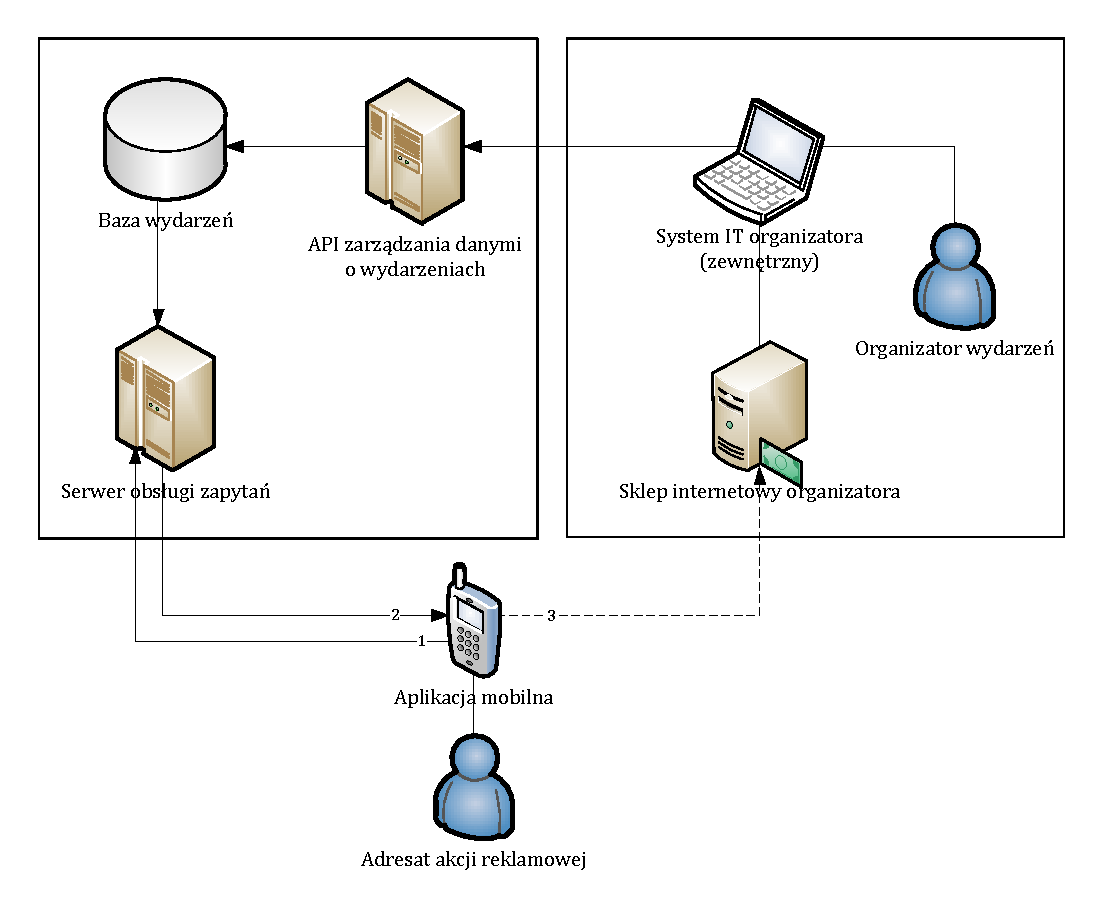
\includegraphics[width=\textwidth]{./figury/produkty/schemat-wspolpracy}
    \caption{Schemat współpracy wszystkich produktów technicznych projektu.}
    \label{fig:produkty:schemat_wspolpracy}
\end{figure}
